%coding:utf-8

%----------------------------------------
%FOSAPHY, a LaTeX-Code for a summary of linear systems and regulation
%Copyright (C) 2014, Mario Felder, Michael Fallegger

%This program is free software; you can redistribute it and/or
%modify it under the terms of the GNU General Public License
%as published by the Free Software Foundation; either version 2
%of the License, or (at your option) any later version.

%This program is distributed in the hope that it will be useful,
%but WITHOUT ANY WARRANTY; without even the implied warranty of
%MERCHANTABILITY or FITNESS FOR A PARTICULAR PURPOSE.  See the
%GNU General Public License for more details.
%----------------------------------------

\chapter{Regelungstechnik}

\section{Regelkreis}
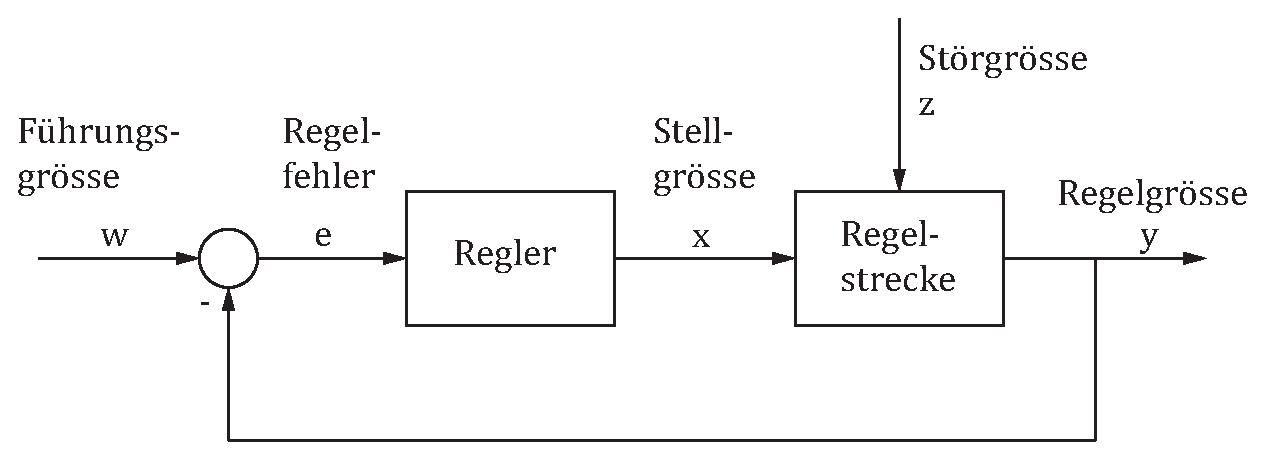
\includegraphics[width = \linewidth]{images/regelkreis.eps}
\\\\
Merkmale:
\begin{itemize}
	\item Erfassen der Regelgrösse $y$
	\item Vergleich von Führungs- und Regelgrösse
	\item Angleichen der Regelgrösse an die Führungsgrösse in Wirkungskreis
\end{itemize}


\section{Systeme}
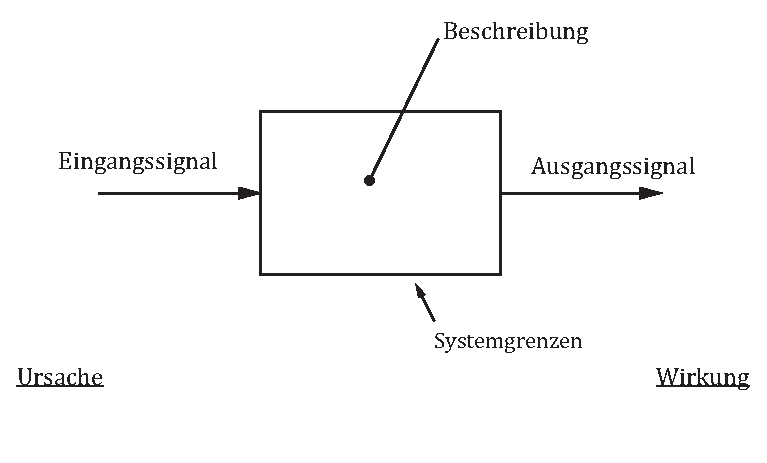
\includegraphics[width = \linewidth]{images/systeme.eps}
\\\\
Signale sind rückwirkungsfrei, also eingeprägte Grössen.
\\\\
\begin{center}
	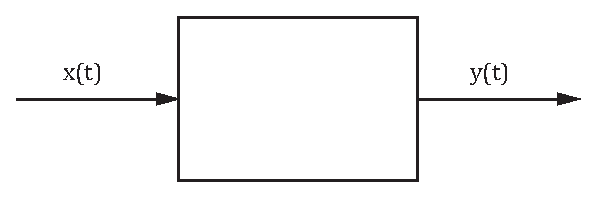
\includegraphics[scale = 0.5]{images/system_bsp.eps}
\end{center}
\begin{tabular}{c|l|l}
 Nr. & Bsp & Klassifikation \\ 
\hline 1 & $y(t) = \cos t \cdot x(t)$ & statisch \\ 
	   2 & $\difrac{y(t)}{t} = - \cos (y(t)) + x(t)$ & \textbf{dynamisch} \\ 
\hline 3 & $\difrac{y(t)}{t} = -y(t) + x(t)$ & \textbf{zeitkontinierlich} \\ 
	   4 & $y((k+1)\tau)=-y(k\cdot \tau) + x(k \cdot \tau)$ & zeitdiskret \\ 
\hline 5 & $y(t) = \cos (x (t-\tau))$ & \textbf{kausal} \\ 
 	   6 & $y(t) = \cos(x(t+\tau))$ & nicht kausal \\ 
\hline 7 & $\difrac{y(t)}{t} = -3y(t) + x(t)$ & \textbf{zeitinvariant} \\ 
	   8 & $\difrac{y(t)}{t} = -\cos t \cdot y(t) +x(t)$ & zeitvariant \\ 
\hline 9 & $\difrac{y(t)}{t} = -y(t) +x(t)$ & \textbf{linear} \\ 
	   10 & $\difrac{y(t)}{t} = -y^2(t) +x(t)$ & nicht linear \\ 
\hline 11 & $\difrac{y(t)}{t} = -y(t) +x(t)$ & \textbf{endlich-dimensional} \\ 
	   12 & $\pdifrac{y(t)}{t} = - \pdifrac{}{x}y(x,t)+x(t)$ & unendlich-dimensional \\ 
\hline 13 & $y(t) = t \cdot \cos^2 t \cdot x(t)$ & \textbf{single input / single output} \\ 
	   14 & $\left[ \begin{matrix} y_1(t) \\ y_2(t) \end{matrix}\right] = \left[ \begin{matrix} -3 & \sin(t) \\ t & -1\end{matrix}\right] \cdot \left[ \begin{matrix} x_1(t)\\ x_2(t) \end{matrix}\right]$ & multiple input / multiple output \\ 
\end{tabular} 
\\\\

\section{Linearisierung}
Approximation durch Gerade:
\[
	f(\bar{x}+\Delta x) \approx \left.(\bar{x})+\difrac{f}{x}\right|_{\bar{x}}\cdot \Delta x
\]

\subsection{Arbeitspunkt festlegen}

Im stationären Zustand gilt:
\[
	\difrac{^n}{t^n} = 0
\]

Für das Eingangssignal $u(t)$ und das Ausgangssignal $y(t)$:
\[
	h(t) = \bar{y} + \Delta y(t) \qquad ,\ u(t) = \bar{u} + \Delta u(t)
\]


\subsection{Linearisierung um Arbeitspunkt}
Es gilt:
\[
	D(y^{(n)}, y^{(n-1)}, \dots ,\dot{y} ,y, u^{(m)}, u^{(m-1)}, \dots , \dot{u} ,u)= 0
\]
$D$ kann am Punkt $\bar{y}, \bar{u}$ approximiert werden durch:
\begin{small}
\[
	\left.\pdifrac{D}{y^{(n)}}\right|_{\begin{scriptsize}\begin{matrix} \bar{y} \\ \bar{u} \end{matrix}\end{scriptsize}} \cdot \Delta y^{n} + \dots +
	\left.\pdifrac{D}{\dot{y}}\right|_{\begin{scriptsize}\begin{matrix} \bar{y} \\ \bar{u} \end{matrix}\end{scriptsize}} \cdot \Delta \dot{y} +
	\left.\pdifrac{D}{y}\right|_{\begin{scriptsize}\begin{matrix} \bar{y} \\ \bar{u} \end{matrix}\end{scriptsize}} \cdot \Delta y +
	\left.\pdifrac{D}{u^{(n)}}\right|_{\begin{scriptsize}\begin{matrix} \bar{y} \\ \bar{u} \end{matrix}\end{scriptsize}} \cdot \Delta u^{n} + \dots +
	\left.\pdifrac{D}{u}\right|_{\begin{scriptsize}\begin{matrix} \bar{y} \\ \bar{u} \end{matrix}\end{scriptsize}} \cdot \Delta u = 0
\]
\end{small}

\begin{center}
	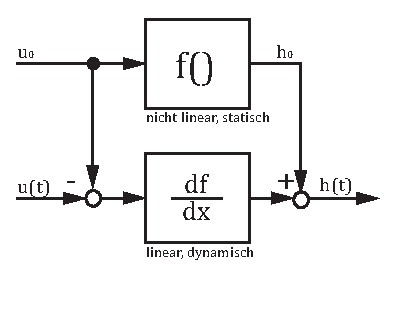
\includegraphics[scale = 0.8]{images/linearisierung.eps}
\end{center}

\section{Stabilität}
Grundlegendes Stabilitätskriterium für LZI-Glieder:\\
\begin{center}
\fbox{\parbox{.9\linewidth}{
	Ein LZI-Glied ist genau dann stabil, wenn die $n$ Nullstellen des Nennerpolynoms sämtliche negative Realteile haben. In der komplexen $s$-Ebene müssen die Nullstellen sämtlich links von der imaginären Achse liegen.
}}
\end{center}

\subsection{Hurwitz-Kriterium}
Das Polynom $N(s) = a_0 + a_1s + a_2s^2 + a_ns^n = 0$ ist nur dann stabil, 
wenn alle Koeffizienten $a_0, a_1, a_2, \ldots a_2$ \uline{ungleich null} sind und
ein \uline{positives Vorzeichen} haben. Zusätzlich müssen alle $n$ \uline{Linieardeterminanten positiv} sein (mit $n$ Zeilen und $n$ Spalten).  
\[
	D_n = \begin{vmatrix}
	a_1 & a_3 & a_5 & a_7 & \ldots \\ 
	a_0 & a_2 & a_4 & a_6 & \ldots \\ 
	0 & a_1 & a_3 & a_5 & \ldots \\ 
	0 & a_0 & a_2 & a_4 & \ldots \\ 
	0 & 0 & a_1 & a_3 & \ldots \\ 
	0 & 0 & a_0 & a_2 & \ldots \\
	\ldots
	\end{vmatrix} 
\]\\
Mit den jeweiligen Unterdeterminanten (für den fall $n=3$):\\
\[\begin{aligned}
	D_1 &= \begin{vmatrix}
		a_1 
		\end{vmatrix} = a_1 > 0\\
	D_2 &= \begin{vmatrix}
		a_1 & a_3 \\
		a_0 & a_2
	\end{vmatrix} = a_1a_2 - a_3a_0 > 0\\
	D_3 &= \begin{vmatrix}
		a_1 & a_3 & 0\\
		a_0 & a_2 & 0\\
		0	& a_1 & a_3
	\end{vmatrix} = a_3 D_2 > 0
\end{aligned}\]\\
Die letzte Determinante erfüllt jeweils zwangsmässig die Bedingung.

\subsection{Nyquist-Kriterium}
Das Nyquist-Kriterium betrachtet die Ortskurve gegenüber dem Punkt $-1$ auf der reelen Achse. Dabei wird die Winkeländerung von $\omega = 0 \rightarrow \omega = \infty$ betrachtet. Dabei muss folgende Beziehung erfüllt sein, damit das Regelsystem stabil ist:
\[
	\Delta \varphi = i_k \cdot \frac{\pi}{2} + r_k \cdot \pi
\]\\
\begin{footnotesize}
	$r_k$: Anzahl Polstellen mit positivem Realteil\\
	$i_k$: Anzahl Polstellen auf der imaginären Achse
\end{footnotesize}

\begin{center}
	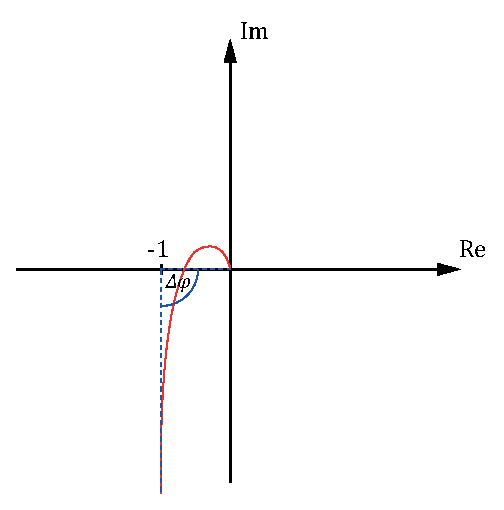
\includegraphics[scale=0.7]{images/nyquist.eps}
\end{center}

\section{Amplituden- und Phasenreserve}
Die Amplitudenreserve $A_R$ ist ein Mass für den Abstand der Ortskurve $G_O(\im\omega)$ vom Punkt $-1$ in Richtung der reelen Achse. Die Kreisfrequenz an der Stelle, an der $G_O(\im\omega)$ die reelle Achse schneidet, heisst Phasenschnittkreisfrequenz $\omega_\pi$.\\
Definition Amplitudenreserve:
\[
	A_R = \frac{1}{\left|G_O(\im\omega)\right|} \qquad \text{Stabilitätsbedingung: } A_R > 0.
\]\\\\
Die Phasenfrequenz $\varphi_R$ ist der Winkel zwischen der negativ-reellen Achse und dem Punkt, an dem die Ortskurve  $G_O(\im\omega)$ den Einheitskresi schneidet. Die Kreisfrequenz im Schnittpunkt heisst Durchtrittskresifrequenz $\omega_D$.\\
Definition Phasenreserve:
\[
	\varphi_R = \angle{G_O(\im\omega)}} + \pi \qquad \text{Stabilitätsbedingung: } \varphi > 0.
\]\\\\
Ablesen von der Ortskurve:
\begin{center}
	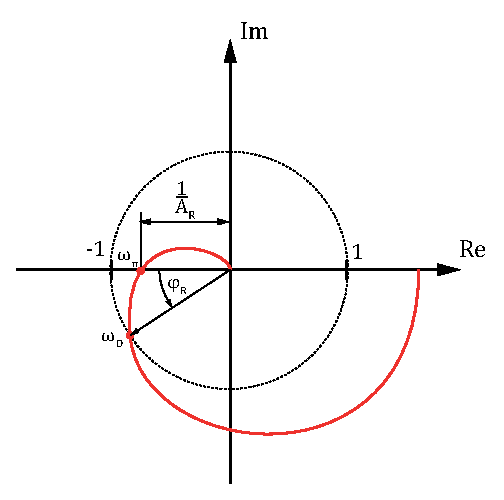
\includegraphics[scale=0.7]{images/ort_reserve.eps}
\end{center}
Ablesen vom Bodediagramm:
\begin{center}
	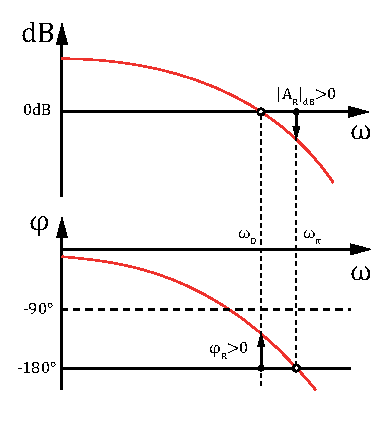
\includegraphics[scale=0.9]{images/bode_reserve.eps}
\end{center}

\subsection{Totzeitreserve}
Die Totzeitreserve $T_{tR}$ ist eine zusätzliche Totzeit, die in einem Regelkreis auftreten darf, ohne dass der Regelkreis instabil wird.\\
Definition Todzeitreserve:
\[
	T_{tR} = \frac{\varphi_R}{\omega_D}
\]
\section{Kompositionen von Grundelementen}

Betrachten der Verkettung:
\begin{center}
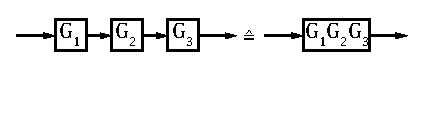
\includegraphics[scale = 1]{images/komp_grnd.eps}
\end{center}
Allgemeine Übertragungsfunktion:
\[
	G(s) = k \frac{s^n \cdot (1+sT_1)^n \ldots}{s^m \cdot (1+sT_2)^m(1+2dTs+s^2T^2)\ldots} \cdot \e^{-sT}
\]

\begin{tabular}{>{\centering\arraybackslash}p{1.5cm}|>{\centering\arraybackslash}p{2.5cm}|>{\centering\arraybackslash}p{2cm}|>{\centering\arraybackslash}p{2.5cm}}
	   \rule[-2ex]{0pt}{5.5ex} Anteil  & Bode  & Ortskurve  & Sprungantwort  \\ 
\hline \rule[-2ex]{0pt}{5.5ex} $k$  & 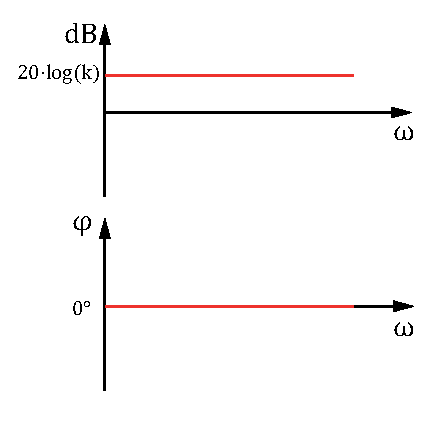
\includegraphics[scale = 0.3]{images/bode_k.eps} & 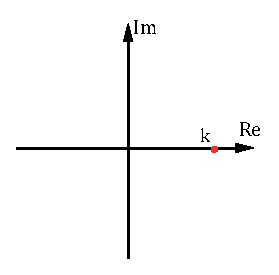
\includegraphics[scale = 0.4]{images/ort_k.eps} & 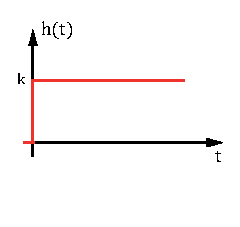
\includegraphics[scale = 0.5]{images/spr_k.eps} \\ 
\hline \rule[-2ex]{0pt}{5.5ex} $s^n$ & 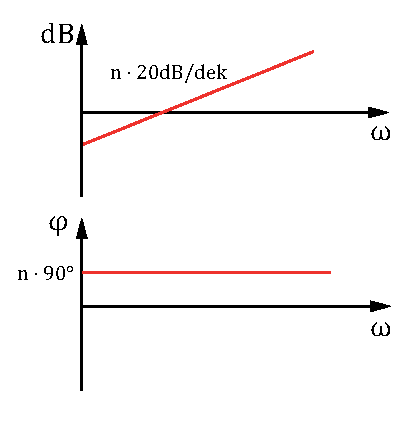
\includegraphics[scale = 0.3]{images/bode_sn.eps} & 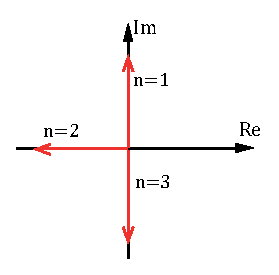
\includegraphics[scale = 0.4]{images/ort_sn.eps}  & 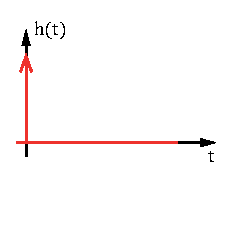
\includegraphics[scale = 0.5]{images/spr_sn.eps}  \\ 
\hline \rule[-2ex]{0pt}{5.5ex} $\frac{1}{s^m}$ & 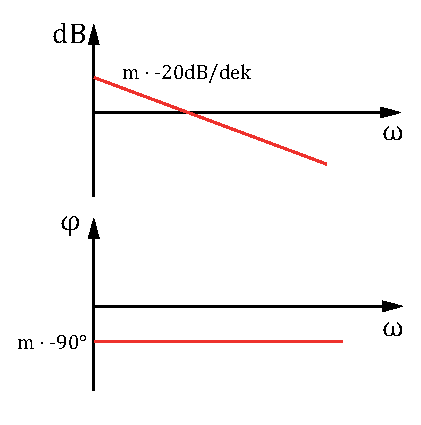
\includegraphics[scale = 0.3]{images/bode_sm.eps}  & 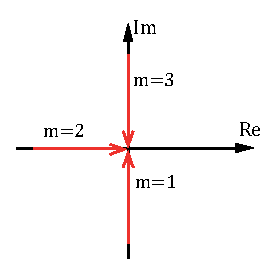
\includegraphics[scale = 0.4]{images/ort_sm.eps}  & 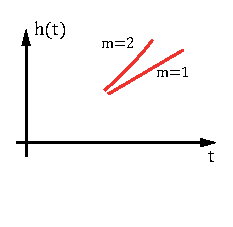
\includegraphics[scale = 0.5]{images/spr_sm.eps} \\ 
\hline \rule[-2ex]{0pt}{5.5ex} $(1+sT)^n$ & 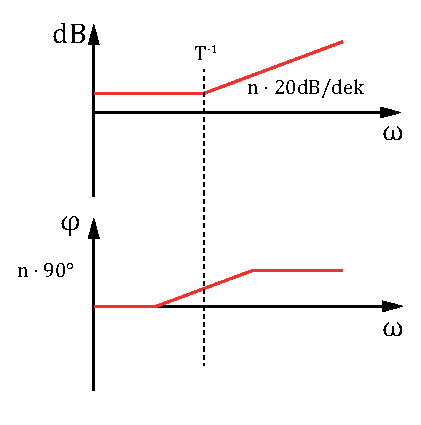
\includegraphics[scale = 0.3]{images/bode_1stn.eps} & 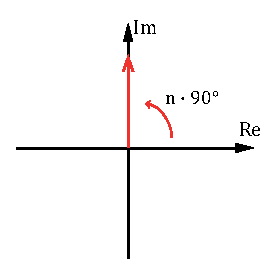
\includegraphics[scale = 0.4]{images/ort_1stn.eps}  & 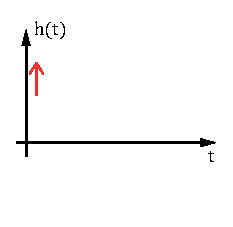
\includegraphics[scale = 0.5]{images/spr_1stn.eps} \\ 
\hline \rule[-2ex]{0pt}{5.5ex} $\frac{1}{(1+sT)^m}$ & 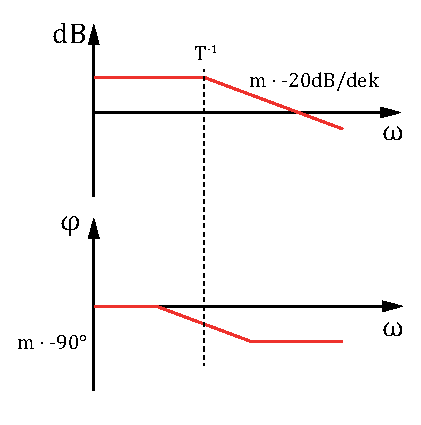
\includegraphics[scale = 0.3]{images/bode_1stm.eps} & 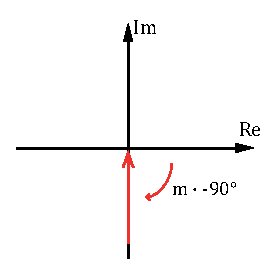
\includegraphics[scale = 0.4]{images/ort_1stm.eps} & 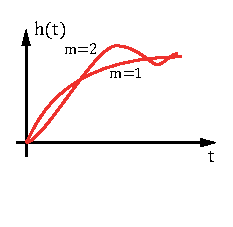
\includegraphics[scale = 0.5]{images/spr_1stm.eps} \\ 
\hline \rule[-2ex]{0pt}{5.5ex} $\e^{-sT}$ & 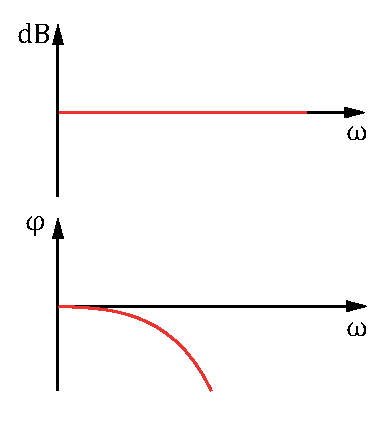
\includegraphics[scale = 0.3]{images/bode_est.eps} & 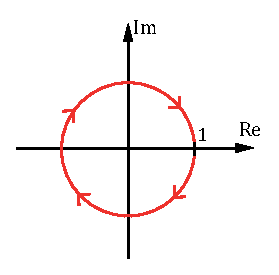
\includegraphics[scale = 0.4]{images/ort_est.eps} & 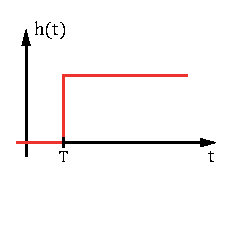
\includegraphics[scale = 0.5]{images/spr_est.eps} \\ 
\end{tabular} 
